\chapter{Fundamentação Teórica}
% Reinicia numeração de tabelas para este capítulo
\setcounter{table}{0}

Este capítulo reúne a fundamentação teórica necessária, cobrindo conceitos de computação em nuvem, virtualização, nuvens privadas, arquitetura do OpenStack e princípios de elasticidade e provisionamento dinâmico de recursos.

\section{Computação em Nuvem (\textit{Cloud Computing})}
\label{sec:cloud-computing}

\subsection{Definição e Paradigma}

A computação em nuvem (\textit{cloud computing}) é definida na publicação especial\,800--145 do \textit{National Institute of Standards and Technology} (NIST) como um modelo que viabiliza o acesso, pela rede e sob demanda, a um conjunto compartilhado de recursos computacionais configuráveis — redes, servidores, armazenamento, aplicações e serviços. Esses recursos podem ser rapidamente provisionados ou liberados com mínimo esforço de gestão ou interação com o provedor de serviços \cite{mell2011}. Da definição derivam cinco características essenciais:

\begin{itemize}
    \item \textbf{Autoatendimento sob demanda (\textit{On-demand self-service})}: o próprio usuário pode provisionar recursos, como tempo de CPU ou armazenamento, sempre que necessário, sem intervenção humana junto ao provedor \cite{mell2011};
    \item \textbf{Acesso amplo à rede (\textit{Broad network access})}: os serviços são acessíveis via internet por meio de mecanismos padronizados, compatíveis com múltiplos dispositivos \cite{mell2011};
    \item \textbf{Agrupamento de recursos (\textit{Resource pooling})}: processamento, memória, armazenamento e largura de banda são agrupados e redistribuídos dinamicamente entre múltiplos inquilinos (\textit{multi-tenant}) conforme a demanda \cite{mell2011};
    \item \textbf{Elasticidade rápida (\textit{Rapid elasticity})}: a capacidade de hardware aparenta ser ilimitada, podendo aumentar ou diminuir de forma ágil — muitas vezes automática — para acompanhar variações de carga \cite{mell2011};
    \item \textbf{Serviço mensurado (\textit{Measured service})}: o uso de recursos é monitorado, controlado e relatado, garantindo transparência ao provedor e ao consumidor \cite{mell2011}.
\end{itemize}

\subsection{Modelos de Serviço}

Com base nessas características, o NIST classifica os serviços em três modelos:

\begin{description}
    \item[Software como Serviço (SaaS)] oferece aplicações completas hospedadas na nuvem e acessadas pela internet. O usuário não gerencia a infraestrutura subjacente \cite{mell2011};
    \item[Plataforma como Serviço (PaaS)] provê um ambiente na nuvem para que o consumidor implante aplicações próprias, sem administrar servidores, rede ou sistemas operacionais \cite{mell2011};
    \item[Infraestrutura como Serviço (IaaS)] disponibiliza recursos fundamentais — processamento, armazenamento e rede — permitindo ao usuário instalar sistemas operacionais e aplicações com controle limitado de rede \cite{mell2011}.
\end{description}

\begin{figure}[htb]
    \centering
    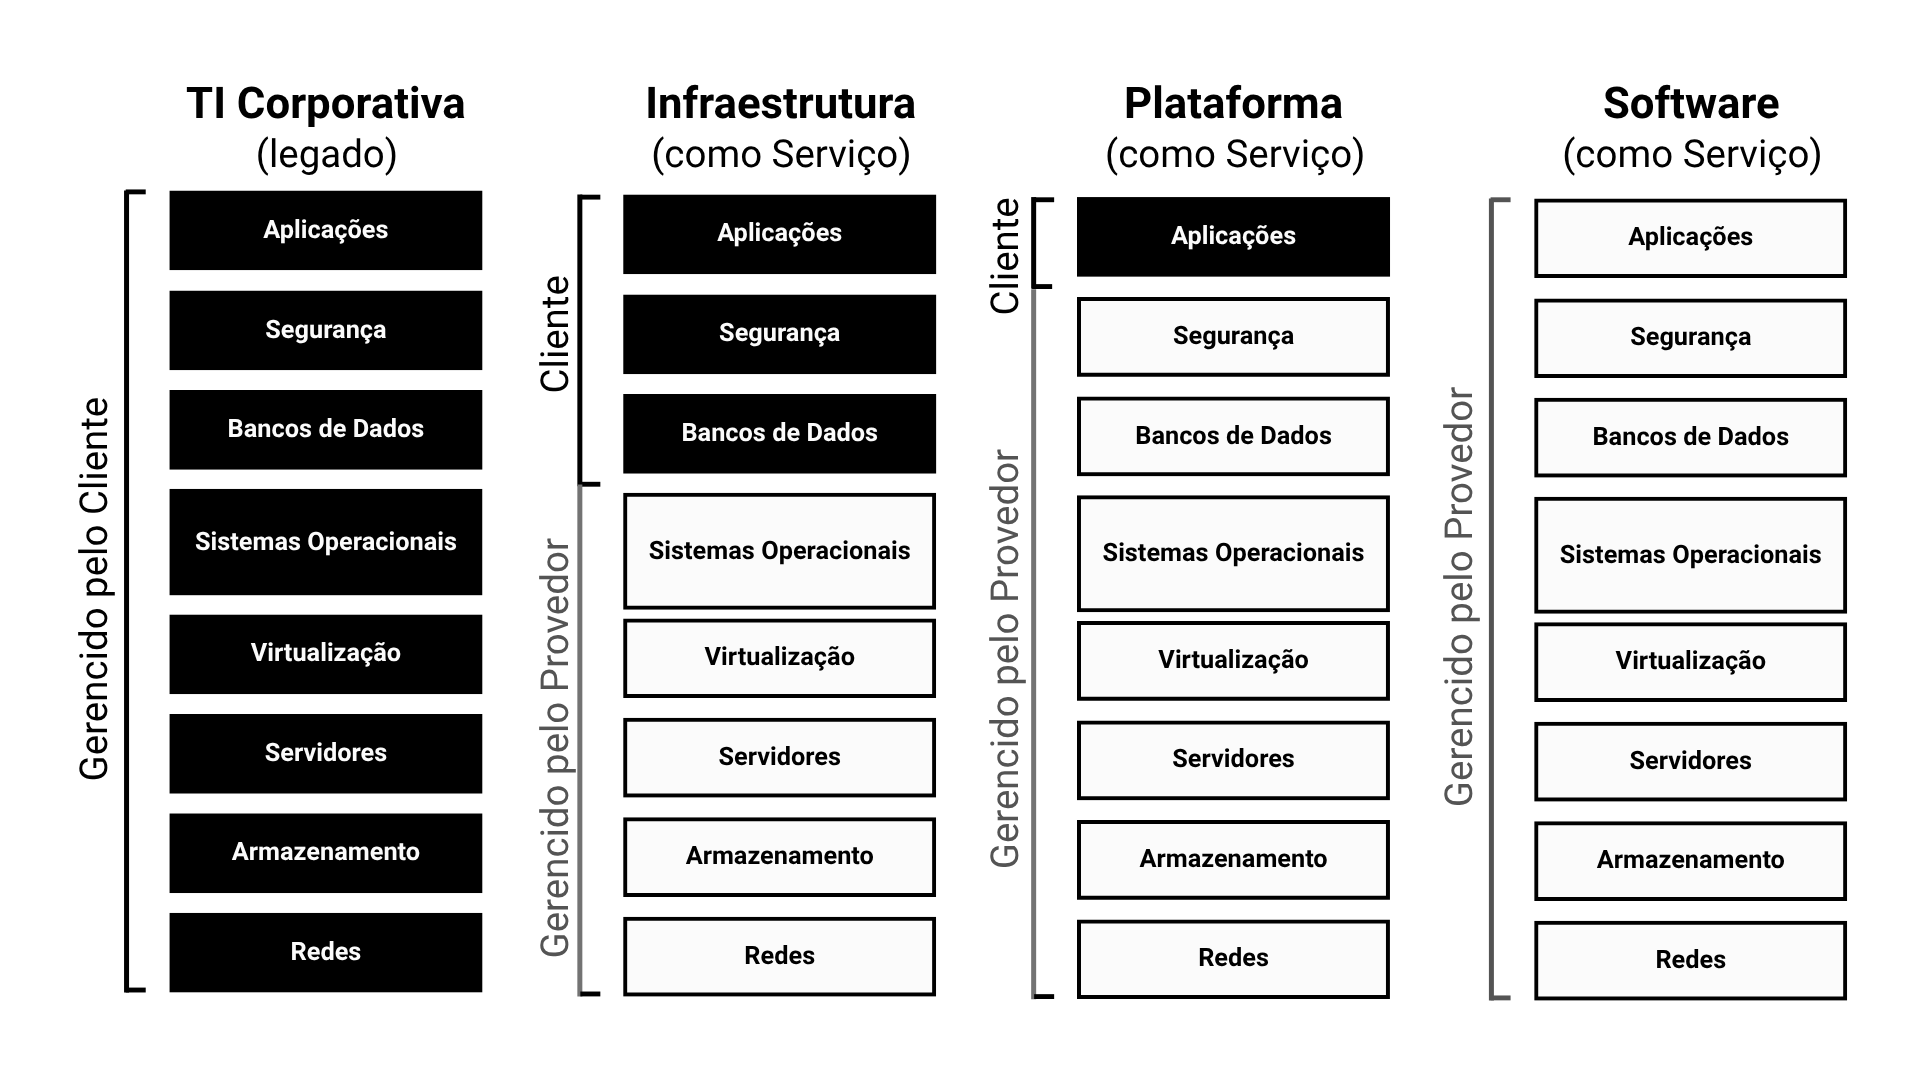
\includegraphics[width=0.8\textwidth]{figuras/Figura 1 - Comparação entre os modelos de serviço.png}
    \caption{Comparação entre os modelos de serviço \textit{IaaS}, \textit{PaaS} e \textit{SaaS}. Adaptado de \cite{rizvi2024}}
    \label{fig:comparacao-modelos-servico}
\end{figure}

A Figura~\ref{fig:comparacao-modelos-servico} sintetiza os níveis de responsabilidade de usuário e provedor em cada modelo. Em SaaS, todo o ciclo da aplicação é responsabilidade do provedor, o que explica sua adoção massiva em redes sociais (\textit{Instagram}, \textit{TikTok}, \textit{WhatsApp}) e serviços de \textit{streaming} (\textit{YouTube}, \textit{Netflix}, \textit{Spotify}) \cite{rizvi2024}. Já o PaaS entrega um ambiente gerenciado de desenvolvimento e implantação, utilizado por soluções como \textit{Microsoft Azure}, \textit{Google App Engine} e \textit{Heroku} \cite{rizvi2024}. No modelo IaaS, o consumidor gerencia sistemas operacionais e middleware sobre recursos virtuais — exemplificados por \textit{AWS EC2/S3}, \textit{Azure Virtual Machines} e \textit{Google Compute Engine} \cite{rizvi2024}.


A computação em nuvem (\textit{cloud computing}) é definida pelo \textit{National Institute of Standards and Technology}(NIST), como um modelo que permite acesso a um conjunto compartilhado de recursos computacionais configuráveis, como redes, servidores, armazenamento, aplicações e serviços,  sob demanda e via rede. Esses recursos podem ser rapidamente provisionados e liberados com mínimo esforço de gerenciamento ou interação com o provedor de serviços \cite{mell2011}. Essa definição enfatiza características essenciais da computação em nuvem, dentre as quais destacam-se: 
\textbf{Autoatendimento sob demanda (\textit{On-demand self-service}):} o usuário pode provisionar recursos computacionais, como tempo de servidor e armazenamento em rede, conforme a necessidade, automaticamente e sem necessidade de interação humana com cada provedor de serviço.
\textbf{Acesso amplo à rede (\textit{Broad network access}):} Os serviços da nuvem podem ser acessados pela grande maioria de aparelhos que possuem acesso à internet, com interfaces padronizadas que facilitam a experiência dos usuários que já estão acostumados com algum serviço na nuvem.
 
\textbf{Agrupamento de recursos (\textit{Resource pooling}):} Os recursos computacionais, como processamento, memória, armazenamento e largura de banda de rede, são agrupados pelo provedor para atender múltiplos inquilinos usando um modelo de multilocação (\textit{multi-tenant}), com diferentes recursos sendo distribuídos dinamicamente e redistribuídos conforme a demanda do inquilino.
\textbf{Elasticidade rápida (\textit{Rapid elasticity}):} Os recursos podem ser provisionados e liberados elasticamente, em alguns casos automaticamente, para escalar rapidamente conforme a demanda. Para o usuário, as capacidades disponíveis para provisionamento parecem ser ilimitadas, a depender da quantidade de hardware que o provedor possui,  e podem ser utilizadas em qualquer quantidade, a qualquer momento. 
\textbf{Serviço mensurado (\textit{Measured service}):} Sistemas de nuvem controlam e otimizam automaticamente o uso de recursos utilizando recursos de medição. Devido a isso, o uso dos recursos pode ser monitorado, controlado e reportado, proporcionando transparência tanto para o provedor quanto para o consumidor do serviço utilizado. 

Além dessas características essenciais, os serviços oferecidos por provedores de nuvem são classificados em modelos de serviço:

\textbf{Software como Serviço (\textit{SaaS})}: é um modelo de distribuição de software onde o software é hospedado na nuvem e disponibilizado aos usuários através da internet. Essa infraestrutura de nuvem é formada por uma camada física, composta por servidores, armazenamento e componentes de rede, e uma camada de abstração, que seria um software implantado sobre essa infraestrutura física \cite{mell2011}. 

\textbf{Plataforma como Serviço (\textit{PaaS})}: é um modelo que fornece ao consumidor a possibilidade de implantar, sobre a infraestrutura de nuvem, aplicações criadas ou adquiridas usando linguagens de programação, bibliotecas, serviços e ferramentas compatíveis com o ambiente oferecido pelo provedor. O consumidor não gerencia nem controla a infraestrutura subjacente da nuvem, como redes, servidores, sistemas operacionais ou armazenamento, mas possui controle sobre as aplicações implantadas e, possivelmente, sobre as configurações do ambiente onde essas aplicações serão hospedadas \cite{mell2011}.

\textbf{Infraestrutura como Serviço (\textit{IaaS})}: é um modelo que fornece ao consumidor a capacidade de provisionar recursos computacionais, como processamento, armazenamento, redes e outros, permitindo que ele implante e execute softwares, incluindo sistemas operacionais e aplicações. O consumidor também não gerencia nem controla a infraestrutura física da nuvem, mas tem controle sobre os sistemas operacionais, o armazenamento, as aplicações implantadas e, em alguns casos, controle limitado de componentes específicos de rede, como firewalls do host \cite{mell2011}.

\begin{figure}[htb]
    \centering
    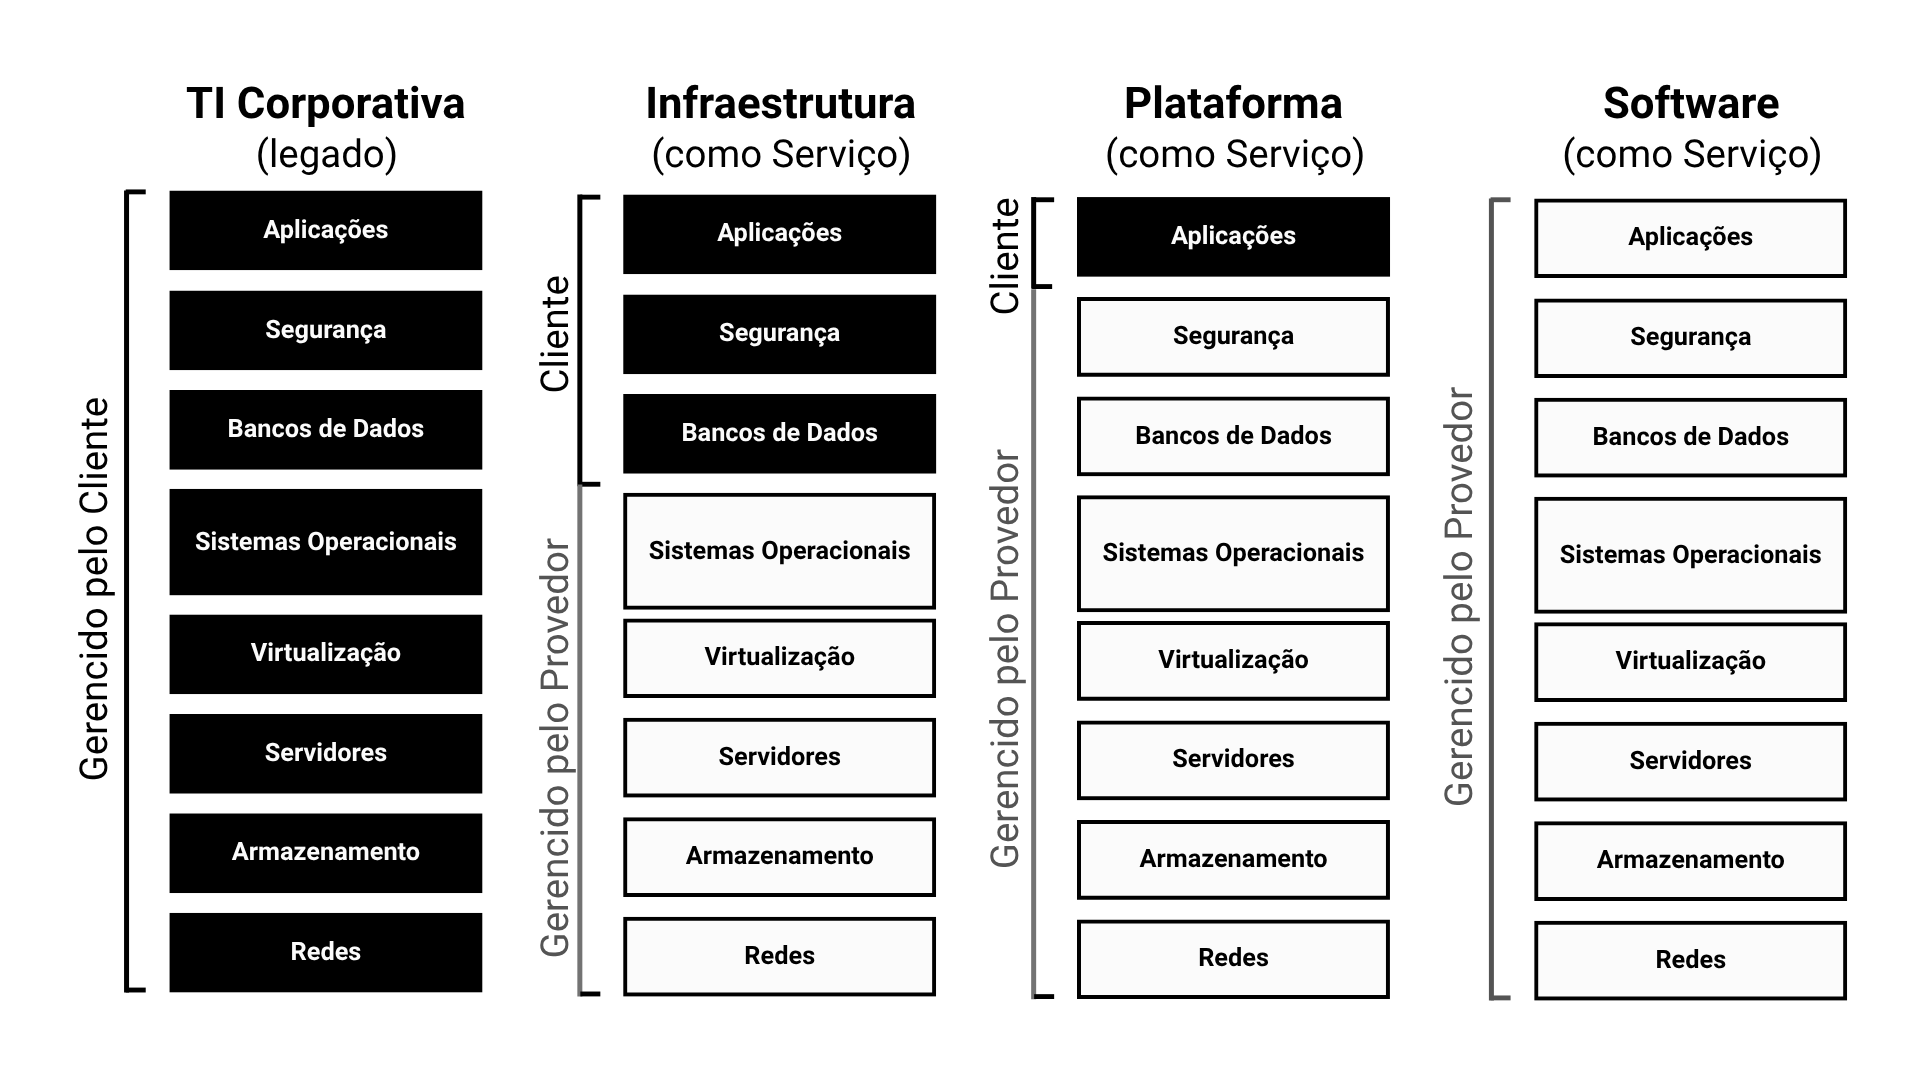
\includegraphics[width=0.8\textwidth]{figuras/Figura 1 - Comparação entre os modelos de serviço.png}
    \caption{Comparação entre os modelos de serviço \textit{IaaS}, \textit{PaaS} e \textit{SaaS}}
    \label{fig:comparacao-modelos-servico}
\end{figure}

Para facilitar o entendimento desses serviços, a Figura \ref{fig:comparacao-modelos-servico} compara os modelos entre si e quais partes da nuvem o usuário tem controle em cada um. Os quadrados verdes representam responsabilidades do usuário, enquanto os azuis são responsabilidades do provedor. Em sistemas de \textit{SaaS}, o usuário não tem responsabilidade nenhuma, mas, em compensação, não gerencia nem controla a infraestrutura da nuvem. Grande parte dos serviços oferecidos a usuários da internet utilizam esse modelo. Dentre eles, pode-se listar as redes sociais, como o \textit{Instagram}, \textit{TikTok} e \textit{Whatsapp}, e serviços de transmissão contínua de conteúdo multimídia (\textit{streaming}), como o \textit{Youtube}, \textit{Netflix} e \textit{Spotify}.  No \textit{PaaS}, o usuário tem controle sobre a aplicação, incluindo códigos e bancos de dados. Nesse modelo encontram-se os serviços de desenvolvimento e hospedagem de software, como \textit{AWS Elastic Beanstalk}, \textit{Google App Engine} e \textit{Heroku}. Já no \textit{IaaS}, o usuário pode solicitar uma quantidade de recursos e tem controle sobre o sistema operacional. Nesse modelo estão as máquinas virtuais e serviços de armazenamento, como  \textit{Amazon Web Services (AWS) EC2 e S3},  \textit{Microsoft Azure Virtual Machines} e  \textit{Google Compute Engine}.

\subsection{Modelos de Implantação}

A implantação de sistemas de computação em nuvem pode ser realizada por meio de diferentes modelos, cada qual adequado a cenários específicos. Os modelos mais difundidos são as nuvens pública, privada, comunitária e híbrida, que se diferenciam em nível de controle, segurança, escalabilidade e custo de implantação \cite{mell2011}.

\begin{description}
  \item[\textbf{Nuvem Pública} (\textit{Public cloud})] \hfill \\ As nuvens públicas são gerenciadas por provedores terceirizados e disponibilizam recursos via internet \cite{carroll2011}. Costumam oferecer alta escalabilidade e baixos custos iniciais, favorecendo organizações de perfis variados \cite{amajuoyi2024}. Entretanto, por serem ambientes compartilhados, podem impor riscos à confidencialidade de dados e perda de controle sobre a infraestrutura, sendo mais recomendadas a empresas com menores exigências de segurança \cite{sathya2023}.

  \item[\textbf{Nuvem Privada} (\textit{Private cloud})] \hfill \\ É uma infraestrutura dedicada a uma única organização, podendo estar on-premises ou em instalações de terceiros \cite{mell2011}. Garante maior controle, personalização e níveis mais altos de segurança. Destaca-se em contextos que exigem proteção de propriedade intelectual ou dados sensíveis \cite{swapna2023}.

  \item[\textbf{Nuvem Comunitária} (\textit{Community cloud})] \hfill \\ Infraestrutura compartilhada por um conjunto de organizações com interesses comuns (por exemplo, requisitos regulatórios), podendo ser mantida interna ou externamente \cite{mell2011}.

  \item[\textbf{Nuvem Híbrida} (\textit{Hybrid cloud})] \hfill \\ Combina duas ou mais infraestruturas (pública, privada ou comunitária), permitindo portabilidade de dados e aplicações entre ambientes \cite{mell2011}.
\end{description}
 
A implantação de sistemas de computação em nuvem pode ser realizada por meio de diferentes modelos. Cada modelo possui características peculiares que determinam sua adequação a contextos específicos. Os modelos mais conhecidos são a nuvem pública, privada, comunitária e híbrida, os quais se diferenciam pelo nível de controle, segurança, escalabilidade e custo de implantação \cite{mell2011}.

As nuvens públicas são gerenciadas por provedores terceirizados que disponibilizam recursos computacionais por meio da internet \cite{carroll2011}. Esses provedores costumam oferecer capacidades elevadas de escalabilidade e custos iniciais mais acessíveis, o que os torna atrativos para diferentes perfis de organizações \cite{amajuoyi2024}. Além disso, esse modelo de nuvem pode ser particularmente vantajoso para instituições que não contam com equipes internas especializadas no assunto ou que optam por não direcionar recursos à aquisição e manutenção de infraestrutura física própria. Em função desses benefícios, a adoção da nuvem pública tem apresentado um crescimento contínuo nos últimos anos \cite{amajuoyi2024}. Entretanto, as nuvens privadas podem apresentar desafios relevantes em termos de segurança e controle sobre a infraestrutura física. A nuvem pública é aberta a todos e sem garantia de alto nível de segurança, podendo trazer riscos à confidencialidade dos dados, à proteção de informações estratégicas e à perda ou roubo de dados, sendo uma opção mais adequada para empresas com "baixas preocupações de segurança" \cite{sathya2023}.

Para organizações que desejam um grau elevado de controle, personalização e alto nível de segurança, as nuvens privadas podem se destacar como uma solução adequada \cite{swapna2023}, consistindo em uma infraestrutura dedicada a uma única organização \cite{mell2011}. Isso possibilita o desenvolvimento de um ambiente seguro e adaptado às exigências particulares de instituições que necessitam resguardar pesquisas sigilosas e proteger a propriedade intelectual. 

\section{Virtualização e Hipervisores}

A virtualização é fundamental na computação moderna por abstrair o hardware de servidores físicos e agrupar logicamente seus recursos em \textit{pools}. Esse agrupamento permite a criação de máquinas virtuais (VMs) isoladas em um único host físico \cite{carissimi2008, kominos2017}. Cada VM opera como um sistema autônomo, com sistema operacional, aplicações e serviços de rede próprios, como se fosse um hardware independente \cite{carissimi2008, smith2005}. Esse particionamento lógico dos recursos viabiliza os pilares da computação em nuvem — elasticidade, multilocação e eficiência de custos \cite{chawla2025}.

\subsection{Tipos de Virtualização}

A implementação de VMs de sistema baseia-se, principalmente, em duas técnicas: virtualização total e paravirtualização \cite{carissimi2008}.

\paragraph{Virtualização Total (\textit{Full Virtualization})} Também chamada de \textit{Hardware Virtual Machine} (HVM), cria uma réplica virtual completa do hardware subjacente, permitindo instalar qualquer sistema operacional sem modificar seu kernel \cite{carissimi2008}. O desafio reside na execução de instruções privilegiadas, originalmente tratadas por emulação de software, introduzindo sobrecarga de desempenho. Extensões de processador como \textit{Intel VT-x} e \textit{AMD-V} minimizaram esse custo ao permitir que o SO virtualizado execute instruções privilegiadas diretamente e com segurança, aproximando o desempenho da VM ao do hardware nativo \cite{carissimi2008, chawla2025}.

\paragraph{Paravirtualização (PV)} Nessa técnica, o sistema operacional é adaptado para operar em ambiente virtualizado: o kernel recebe \textit{drivers} específicos que utilizam chamadas diretas ao hipervisor (\textit{hypercalls}) em vez de instruções privilegiadas \cite{carissimi2008}. Ao eliminar a necessidade de interceptação e emulação, a paravirtualização reduz o \textit{overhead} e apresenta desempenho superior quando comparada à virtualização total sem suporte de hardware \cite{carissimi2008}.

% Tabela 1 – Comparativo entre Virtualização Total e Paravirtualização
\begin{table}[htb]
    \centering
    \caption{Comparativo entre Virtualização Total e Paravirtualização}
    \label{tab:comparativo_virtualizacao}
    \begin{tabularx}{\textwidth}{ l >{\RaggedRight}X >{\RaggedRight}X }
        \toprule
        \textbf{Característica} & \textbf{Virtualização Total} & \textbf{Paravirtualização} \\
        \midrule
        Visão do \textit{Guest} & Hardware virtual idêntico ao físico. & API/hardware simplificado, exposto pelo hipervisor. \\
        \addlinespace
        Modificação do SO & Não é necessária. & Sim, o \textit{kernel} precisa de drivers e \textit{hypercalls} especiais. \\
        \addlinespace
        Instruções Privilegiadas & Interceptadas pelo hipervisor ou tratadas via hardware (\textit{Intel VT-x/AMD-V}). & O \textit{guest} realiza \textit{hypercalls} diretas ao hipervisor. \\
        \addlinespace
        Desempenho & Historicamente mais lento, mas hoje quase nativo graças à assistência de hardware. & Menor sobrecarga e desempenho superior, especialmente em I/O. \\
        \addlinespace
        Principal Vantagem & Compatibilidade universal com qualquer sistema operacional. & Velocidade e eficiência, sobretudo antes da popularização do \textit{Intel VT-x}. \\
        \addlinespace
        Principal Desvantagem & Maior sobrecarga sem assistência de hardware. & Requer suporte e modificação no sistema operacional convidado. \\
        \bottomrule
    \end{tabularx}
    \fonte{Elaborado pelo autor, com base em Carissimi (2008).}
\end{table}

% 2.2.2 – Definição e tipos de hipervisores
\subsection{Hipervisores: Definição e Tipos}

O componente de software responsável por criar e gerenciar máquinas virtuais é denominado \textit{hipervisor} ou Monitor de Máquina Virtual (\textit{Virtual Machine Monitor} — VMM) \cite{chawla2025, carissimi2008}. Posicionado entre o hardware e os sistemas operacionais, ele arbitra o acesso aos recursos físicos e preserva o isolamento entre VMs \cite{chawla2025}.

Os hipervisores são tradicionalmente classificados em dois tipos, conforme ilustrado na Figura~\ref{fig:arq-hipervisores}.

\begin{figure}[htb]
    \centering
    % Substitua pelo caminho correto da imagem
    \includegraphics[width=0.8\textwidth]{figuras/hipervisores_tipo1_tipo2.png}
    \caption{Arquiteturas de hipervisores Tipo 1 e Tipo 2. Adaptado de \cite{chawla2025, kominos2017}}
    \label{fig:arq-hipervisores}
\end{figure}

\paragraph{Tipo 1 (\textit{Bare-Metal})} Executa diretamente sobre o hardware do servidor, atuando como um sistema operacional enxuto dedicado à execução de VMs \cite{chawla2025}. São exemplos o \textit{Xen}, \textit{VMware ESXi} e \textit{Microsoft Hyper-V} \cite{chawla2025, carissimi2008}. Acesso direto ao hardware resulta em melhor desempenho e maior segurança.

\paragraph{Tipo 2 (\textit{Hosted})} Opera como aplicação sobre um sistema operacional convencional (hospedeiro) que gerencia o hardware \cite{chawla2025}. Entre os exemplos estão o \textit{KVM}, \textit{Oracle VirtualBox} e \textit{VMware Player} \cite{chawla2025, carissimi2008}. A instalação é mais simples, porém existe sobrecarga adicional devido à camada do SO hospedeiro.

Para destacar suas diferenças, a Tabela~\ref{tab:comparativo_hipervisores} resume as principais características de cada tipo.

\begin{figure}[htb]
    \centering
    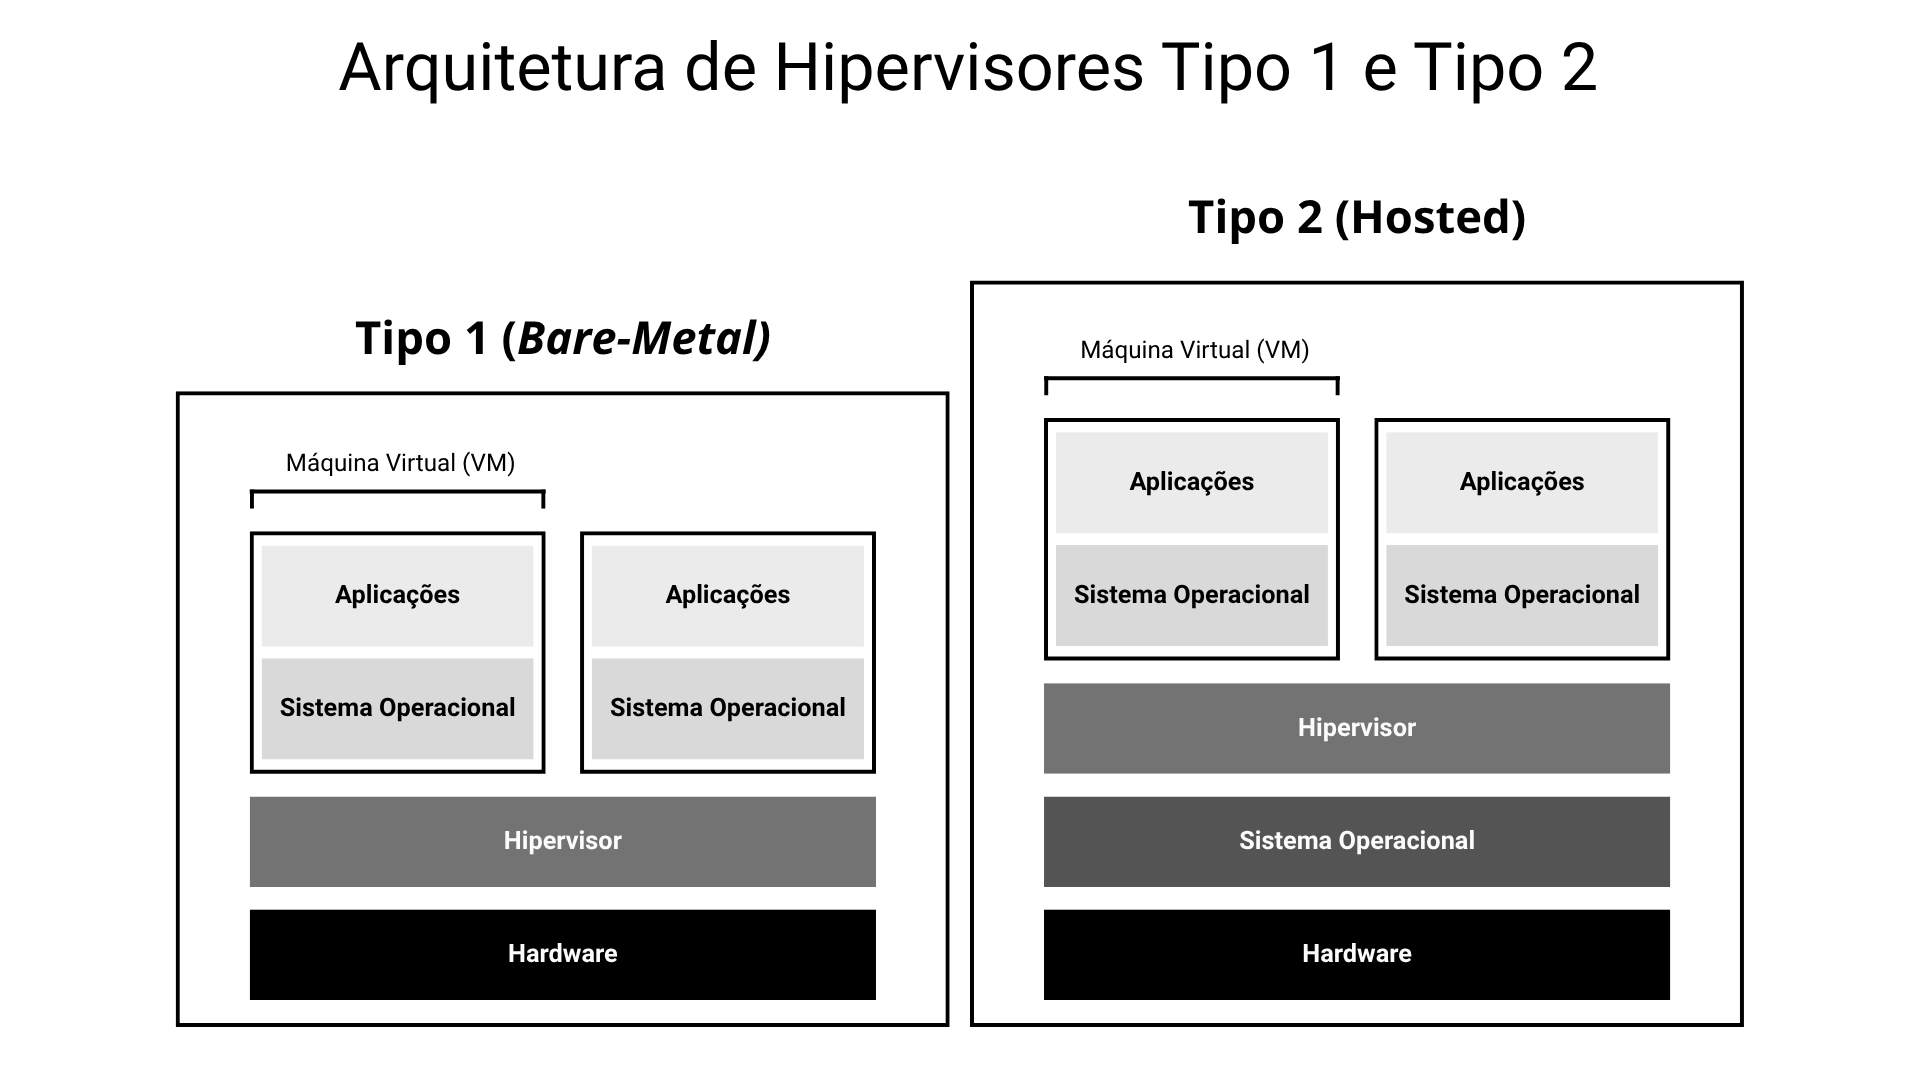
\includegraphics[width=0.8\textwidth]{../figuras/Figura 2 - Arquitetura de Hipervisores.png}
    \caption{Arquitetura típica de hipervisores Tipo 1 e Tipo 2}
    \label{fig:arq_hipervisores}
    \fonte{Imagem adaptada de Chawla et al. (2025) e Kominos, Seyvet e Vandikas (2017).}
\end{figure}

% Tabela 2 – Comparativo entre Hipervisores Tipo 1 e Tipo 2
\begin{table}[htb]
    \centering
    \caption{Comparativo entre Hipervisores Tipo 1 e Tipo 2}
    \label{tab:comparativo_hipervisores}
    \begin{tabularx}{\textwidth}{ >{\bfseries}l >{\RaggedRight}X >{\RaggedRight}X }
        \toprule
        & \textbf{Hipervisor Tipo 1 (Bare-Metal)} & \textbf{Hipervisor Tipo 2 (Hosted)} \\
        \midrule
        Posicionamento Arquitetural & Executa diretamente sobre o hardware físico. & Executa como uma aplicação sobre um Sistema Operacional hospedeiro. \\
        \addlinespace
        Desempenho & Maior, com menor sobrecarga de virtualização. & Menor, pois há uma camada extra (SO hospedeiro) que pode gerar \textit{overhead}. \\
        \addlinespace
        Segurança & Maior — superfície de ataque reduzida. & Menor — depende da segurança do SO hospedeiro. \\
        \addlinespace
        Complexidade de Gerência & Requer conhecimentos especializados. & Geralmente mais simples de configurar. \\
        \addlinespace
        Casos de Uso Típicos & Data centers, nuvens públicas/privadas. & Estações de trabalho, ambientes de teste/desenvolvimento. \\
        \bottomrule
    \end{tabularx}
    \fonte{Elaborado pelo autor com base em Chawla et al. (2025) e Carissimi (2008).}
\end{table}


% 2.2.3 – Análise Comparativa de Hipervisores
\subsection{Análise Comparativa de Hipervisores}

A seleção de um hipervisor impacta diretamente o desempenho, a segurança e a escalabilidade de uma infraestrutura de nuvem. A Tabela~\ref{tab:analise-hipervisores} apresenta a comparação de sobrecarga (\textit{overhead}) em CPU, memória, disco e rede, bem como um índice agregado de desempenho geral, compilada a partir de estudos recentes \cite{chawla2025}.

\begin{table}[htb]
    \centering
    \caption{Desempenho comparado de hipervisores}
    \label{tab:analise-hipervisores}
    \begin{tabularx}{\textwidth}{ >{\bfseries}l c c c c c }
        \toprule
        Hipervisor & CPU (\%) & Memória (\%) & Disco I/O (\%) & Rede (\%) & Índice Geral (0--100) \\
        \midrule
        VMware ESXi & 2,0 & 2,9 & 2,8 & 2,5 & 92 \\
        KVM & 3,5 & 3,0 & 3,8 & 3,5 & 88 \\
        Xen & 4,2 & 4,1 & 4,5 & 4,0 & 81 \\
        Microsoft Hyper-V & 5,0 & 4,5 & 5,0 & 4,5 & 78 \\
        \bottomrule
    \end{tabularx}
    \fonte{Elaborado pelo autor com base em Chawla et al. (2025).}
\end{table}

Observa-se que o \textit{VMware ESXi} apresenta as menores sobrecargas em todas as métricas, refletindo o melhor desempenho global. O KVM surge como alternativa de código aberto competitiva, com eficiência próxima ao ESXi. Já os hipervisores \textit{Xen} e \textit{Hyper-V} exibem sobrecargas superiores, o que pode afetar cargas de trabalho sensíveis a latência e operações de E/S.

% 2.5.2 – Análise Qualitativa de Hipervisores

A Tabela~\ref{tab:hipervisores} resume as principais características, vantagens e desvantagens dos hipervisores analisados, destacando sua aplicabilidade em ambientes de nuvem.

\begin{table}[htb]
    \centering
    \renewcommand{\arraystretch}{1.3}
    \caption{Comparação entre hipervisores KVM, VMware ESXi e Xen}
    \label{tab:hipervisores}
    \begin{tabularx}{\textwidth}{|>{\raggedright\arraybackslash}p{3cm}|X|X|X|}
        \hline
        \textbf{Característica} & \textbf{KVM} & \textbf{VMware ESXi} & \textbf{Xen} \\ \hline
        \textbf{Tipo} & Tipo 2, mas com comportamento de Tipo 1 & Tipo 1 & Tipo 1 \\ \hline
        \textbf{Licença} & Código Aberto & Proprietário & Código Aberto \\ \hline
        \textbf{Vantagens} &
        \begin{itemize}
            \item Desempenho próximo ao nativo.
            \item Custo zero de licenciamento.
            \item Amplo suporte da comunidade \textit{open-source}.
        \end{itemize} &
        \begin{itemize}
            \item Desempenho de E/S superior.
            \item Ecossistema de gerenciamento maduro.
            \item Segurança robusta.
        \end{itemize} &
        \begin{itemize}
            \item Arquitetura de segurança confiável.
            \item Bom isolamento entre VMs.
            \item Ampla adoção em nuvens públicas (AWS).
        \end{itemize} \\ \hline
        \textbf{Desvantagens} &
        \begin{itemize}
            \item Segurança depende do \textit{kernel} Linux.
            \item Gerenciamento menos centralizado.
        \end{itemize} &
        \begin{itemize}
            \item Custo de licenciamento elevado.
        \end{itemize} &
        \begin{itemize}
            \item Maior sobrecarga de desempenho em alguns cenários.
            \item Configuração mais complexa.
        \end{itemize} \\ \hline
    \end{tabularx}
    \fonte{Elaborado pelo autor com base em Chawla et al. (2025), Kominos, Seyvet e Vandikas (2017) e Arora et al. (2014).}
\end{table}

% 2.2.4 – KVM como Solução de Hipervisor
\subsection{KVM como Solução de Hipervisor}

O \textit{Kernel-based Virtual Machine} (KVM) integra um hipervisor diretamente ao \textit{kernel} do \textit{Linux} \cite{carissimi2008}. Embora seja classificado como hipervisor Tipo~2, sua estreita integração com o núcleo do sistema lhe confere desempenho e eficiência próximos aos de hipervisores Tipo~1 \cite{chawla2025, kominos2017}. Cada máquina virtual é executada como um processo convencional, agendado pelo escalonador padrão do \textit{Linux}, otimizando a gestão de CPU e memória \cite{anand2013}.

O KVM explora extensões de virtualização assistida por hardware — Intel VT-x e AMD-V — minimizando a sobrecarga de tradução binária e permitindo que o código privilegiado seja executado diretamente no processador \cite{chawla2025, carissimi2008}. Dessa forma, estudos relatam sobrecarga de CPU em torno de 4\% para o KVM, índice competitivo frente a soluções proprietárias \cite{chawla2025}. Como parte do \textit{kernel} \textit{Linux}, o KVM herda evoluções do subsistema de memória, escalonamento e suporte a novos dispositivos, acompanhando automaticamente os avanços do projeto principal \cite{anand2013, arora2014}.

Em contrapartida, a superfície de ataque do KVM está diretamente relacionada ao tamanho e à segurança do \textit{kernel} \textit{Linux}. Vulnerabilidades no \textit{kernel} podem levar a ataques como \textit{VM escape} ou \textit{hyperjacking}. Hipervisores com \textit{microkernel} próprio, como o \textit{VMware ESXi} e o Xen, apresentam uma base de código menor e, consequentemente, área de ataque reduzida, sendo preferidos em ambientes que demandam requisitos de segurança mais rigorosos \cite{chawla2025}.

\section{Máquinas Virtuais \& Imagens}

% 2.3 – OpenStack
\section{OpenStack}

% 2.3.1 – Definição e Características
\subsection{Definição e Características}

O \textit{OpenStack} é uma plataforma de código aberto voltada à construção e ao gerenciamento de nuvens no modelo \textit{Infrastructure as a Service} (IaaS). Surgiu em 2010 como iniciativa conjunta da \textit{Rackspace Inc.} — que possuía um serviço de armazenamento de objetos escalável — e da \textit{NASA}, que buscava atender às suas demandas computacionais por meio do projeto Nebula \cite{nasa2012}. Ambas disponibilizaram o código sob licença \textit{Apache~2.0}, fomentando uma comunidade global de desenvolvimento.

A adoção do OpenStack deve-se à natureza aberta, flexível e de baixo custo de licenciamento. Sua arquitetura modular permite implantar apenas os serviços necessários — computação (\textit{Nova}), armazenamento de objetos (\textit{Swift}), rede (\textit{Neutron}), entre outros — e personalizar funções para requisitos específicos \cite{grzonka2015}. A combinação de escalabilidade massiva, apoio da comunidade e participação de grandes empresas faz do OpenStack a escolha de data centers, operadoras de telecomunicações e instituições de pesquisa, como o CERN \cite{rousseau2019}.

% 2.3.2 – Módulos para configurações básicas do OpenStack
\subsection{Módulos Básicos do OpenStack}

Por compor-se de diversos projetos independentes, o OpenStack permite selecionar módulos conforme a necessidade. Contudo, alguns se destacam como base da maioria das implantações:

\begin{itemize}
    \item \textbf{Nova}: serviço de computação responsável pela criação, dimensionamento e destruição de instâncias de máquinas virtuais.
    \item \textbf{Neutron}: provê abstração e orquestração de redes virtuais, oferecendo conectividade \textit{L2/L3}, balanceamento de carga e \textit{firewalls}.
    \item \textbf{Glance}: catálogo e serviço de gerenciamento de imagens de discos utilizados para inicializar VMs.
    \item \textbf{Keystone}: serviço de identidade que centraliza autenticação, autorização e catálogo de endpoints.
    \item \textbf{Horizon}: painel web que oferece interface gráfica para administrar os serviços OpenStack.
    \item \textbf{Cinder}: volume block storage que disponibiliza armazenamento persistente, independente do ciclo de vida das instâncias.
    \item \textbf{Swift}: armazenamento de objetos distribuído, altamente escalável.
\end{itemize}

% --- Detalhamento dos módulos ---
\subsubsection{Keystone: Serviço de Identidade}

O \textit{Keystone} fornece autenticação, autorização e catálogo de serviços no ecossistema OpenStack \cite{openstack_keystone}. Seus principais recursos incluem:
\begin{itemize}
    \item \textbf{Autenticação}: múltiplos métodos (senha, tokens, federado, LDAP) para validar usuários e serviços.
    \item \textbf{Autorização}: políticas baseadas em funções que controlam o acesso a projetos, usuários e grupos.
    \item \textbf{Catálogo de Serviços}: lista endpoints REST dos serviços registrados, permitindo descoberta dinâmica.
    \item \textbf{Gerenciamento de Usuários e Grupos}: criação e manutenção de domínios, projetos, usuários e grupos.
\end{itemize}

\subsubsection{Nova: Serviço de Computação}

O \textit{Nova} orquestra o ciclo de vida das instâncias de máquinas virtuais ou contêineres \cite{openstack_nova}. Funcionalidades principais:
\begin{itemize}
    \item \textbf{Gerenciamento de Instâncias}: operações de criação, parada, reinicialização, migração e exclusão.
    \item \textbf{Agendamento de Recursos}: algoritmo pluggable que seleciona o \textit{compute node} ideal com base em filtros de capacidade e afinidade.
    \item \textbf{Integração com Hipervisores}: suporte a KVM, Xen, VMware ESXi, Hyper-V, entre outros.
    \item \textbf{APIs REST}: interface pública e interna para automação e integração com ferramentas de nuvem.
\end{itemize}

\subsubsection{Neutron: Serviço de Rede}

O \textit{Neutron} provê serviços de rede em nível 2/3 e avançados (FWaaS, LBaaS, VPN) \cite{openstack_neutron}. Funcionalidades principais:
\begin{itemize}
    \item \textbf{Gerenciamento de Redes}: criação de redes virtuais, sub-redes, portas e segurança de portas (SG).
    \item \textbf{Roteamento}: gateways externos, roteadores virtuais e NAT para conectividade externa.
    \item \textbf{Firewall as a Service}: políticas de segurança de tráfego ingress/egress.
    \item \textbf{Load Balancing as a Service}: balanceamento L4 e L7 com alta disponibilidade.
    \item \textbf{Integração SDN}: compatibilidade com Open vSwitch, OVN, Calico e controladores SDN.
\end{itemize}

\subsubsection{Horizon: Dashboard}

O \textit{Horizon} fornece uma interface web unificada para usuários e administradores \cite{openstack_horizon}. Principais capacidades:
\begin{itemize}
    \item \textbf{Interface Gráfica}: acesso visual a todos os serviços sem CLI.
    \item \textbf{Gerenciamento de Recursos}: instâncias, volumes, redes, imagens e identidades.
    \item \textbf{Monitoramento}: visão do estado e uso de quota dos projetos.
    \item \textbf{Extensibilidade}: framework para criação de painéis customizados.
\end{itemize}

\subsubsection{Glance: Serviço de Imagem}

O \textit{Glance} armazena e distribui imagens de discos de VM \cite{openstack_glance}. Funcionalidades:
\begin{itemize}
    \item \textbf{Registro e Descoberta}: upload, versionamento e busca de imagens.
    \item \textbf{Armazenamento Backend}: drivers para Swift, sistemas de arquivos locais, Ceph, S3.
    \item \textbf{Metadados}: esquema flexível para anexar atributos às imagens.
    \item \textbf{API RESTful}: operações CRUD de imagens e metadados.
\end{itemize}


\section{Elasticidade e Provisionamento Dinâmico}

\subsection{Dimensionamento \textit{automático}}

\subsection{Políticas de \textit{Fair-Share} e \textit{Ballooning}}

\section{Imagens Base Compartilhadas}

\section{Trabalhos Relacionados}

\section{Síntese dos Conceitos}
